\documentclass{article}

\usepackage[margin=1.5in]{geometry}

% Tables
\usepackage{adjustbox}
\usepackage{array}
\usepackage{booktabs}
\usepackage{multirow}

\newcolumntype{R}[2]{%
    >{\adjustbox{angle=#1,lap=\width-(#2)}\bgroup}%
    l%
    <{\egroup}%
}
\newcommand*\rot{\multicolumn{1}{R{0}{1em}}}% no optional argument here, please!
\renewcommand*\rot{}

% Links
\usepackage{hyperref}

% Figures
\usepackage{float}
\usepackage{subcaption}

% Bibliography
\usepackage[
%style=chicago-authordate,
backend=biber,
style=nature,
]{biblatex}

%\usepackage[backend=biber]{biblatex-chicago}  

\addbibresource{bibliography.bib}

% Lists
\usepackage{enumitem}

% Math
\usepackage{amsmath,amsfonts,amssymb}
\DeclareMathOperator*{\argmax}{arg\,max}
\DeclareMathOperator*{\argmin}{arg\,min}

% Algorithms
\usepackage{algorithm, algpseudocode}
\algblock{Input}{EndInput}
\algnotext{EndInput}
\algblock{Output}{EndOutput}
\algnotext{EndOutput}
\newcommand{\Desc}[2]{\State \makebox[2em][l]{#1}#2}

% Inkscape
\usepackage{import}
\usepackage{xifthen}
\usepackage{pdfpages}
\usepackage{transparent}

% Watermark
%\usepackage{background}

\title{What Factors Drive Positive Educational Outcomes in School Districts and How Do We Maximize These?}
\author{Gabriel Bermudez Sellars\\Alejandro Guzman\\Conor Olive\\Mayzee Supak\\Max Woodruff-Maderia}
\date{}

\begin{document}

\maketitle

\tableofcontents

\section{Introduction}

Education is a very important and powerful tool that helps people succeed in life; however, not all education is equal \autocite{doi:10.1177/0013124519833442}. Schools’ education standards and resources vary greatly depending on the local district where students live, which is not fair to students who happen to reside within school districts that create poor student outcomes. Measurable disparity in educational spending remains between school districts in spite of best efforts, and is often linked to persistent \textit{de facto} racial segregation\autocite{kitchens2021} between them.

Our project seeks to first determine which factors best predict positive educational outcomes across school districts. Second, informed by this information, we seek to design school districts which maximize equity in these factors between school districts.

To answer the first question, we use data from the Urban Institute\autocite{urban}, which combines multiple datasets\autocite{urbansources} from the federal government and harmonizes variables across them into one easily accessible dataset. Specific federal data sources collated include
\begin{itemize}
    \item Common Core of Data
    \item EDFacts
    \item The Civil Rights Data Collection
    \item Small Area Income and Poverty Estimates
\end{itemize}
We choose to utilize country-wide data from 2018, one of the recent years in which all sources published reports. We then perform \textit{ordinary least squares} linear regression on the data and analyze the resulting constant coefficients to investigate how different predictors affect the educational outcomes measured in the dataset, namely test scores and graduation rates. We choose this model since we seek to maximize interpretability of the model, rather than accuracy.

To answer the second question, we use data from the U.S. Census, specifically school district geometries, Census block geometries\autocite{censusblocks}, and population by age and sex\autocite{censusblockdata}, provided per Census block for Alameda County in 2020. Also utilized were Alameda County Tax Assessments\autocite{landvalue} for individual parcels in 2020. We then construct a graph and spanning forest representation of the blocks in each school district and perform a greedy optimization routine on the spanning forest to produce a new spanning forest which locally minimizes an objective function that measures variance in identified predictors from the linear model.

In our particular area of focus in Alameda County, there are 522 Census blocks that may belong to any one of 3 possible districts, giving a finite, discrete domain containing \(3^{522}\) possible solutions. By representing the blocks as nodes in a graph with shared borders as edges, we can easily enforce the feasible set of solutions containing only connected districts in our optimizer, and explore the neighborhood of existing solutions (i.e. in the world as they exist now).

\section{Techniques and Methods}
\subsection{Predictors of Educational Outcomes}\label{sec:model}
\subsubsection{Linear Regression}
To perform linear regression, we use an ordinary least squares method in order to find the coefficients \(\hat{\beta}\) in the system
\begin{equation*}
    \mathbf{X}\hat{\beta} = \mathbf{y},
\end{equation*}
where \(\mathbf{X}\) is a matrix with columns representing values in Table \ref{tab:model-x}, and \(\mathbf{y}\) is a matrix with columns representing the variables in Table \ref{tab:model-y}. Each row of \(\mathbf{X}\) and \(\mathbf{y}\) represents a single district. Using the method of ordinary least squares means that we find \(\hat{\beta}\) as 
\begin{equation*}
    \hat{\beta} = \argmin_{\beta}{\left|\left|\mathbf{y}-\mathbf{X}\beta\right|\right|^2}.
\end{equation*}
The library used to perform this is \textit{sklearn.linear\_model.LinearRegression}. In addition, we split the rows of \(\mathbf{X}\) and \(\mathbf{y}\) into training and testing, at a ratio of \(0.7\), and evaluate goodness of fit using mean squared error.

\subsubsection{Data}
To assess what factors determine positive educational outcomes, we perform linear regression on district--level data in 2018 obtained from Urban Institute's Education Data Portal\autocite{urban}. From the various available variables in the data set, we choose, from the ``Edfacts State Assements'' and ``Edfacts Adjusted Cohort Graduation Rates'' to be our dependent variables and the best measures of student outcome in the dataset. These are shown in Table \ref{tab:model-y}
\begin{table}[h]
    \centering
    \begin{tabular}{lp{8cm}}
         \textbf{Name} & \textbf{Description} \\ \hline
         \texttt{math\_test\_pct\_prof\_midpt} & Midpoint of the range used to report the share of students scoring proficient on a mathematics assessment (0--100 scale) \\ \hline
         \texttt{read\_test\_pct\_prof\_midpt} & Midpoint of the range used to report the share of students scoring proficient on a reading or language arts assessment (0--100 scale) \\ \hline
         \texttt{grad\_rate\_midpt} & Midpoint of the high school graduation rate range (0--100 scale)
    \end{tabular}
    \caption{Dependent variables used as a measure of educational outcomes.}
    \label{tab:model-y}
\end{table}

In addition, we choose variables from the ``Common Core of Data'' finance and directory datasets which we hypothesize may well predict dependent variables in Table \ref{tab:model-y}. These values, shown in Table \ref{tab:model-x}, are {divided by \texttt{enrollment} to provide \texttt{per\_student} variables}, which are what is actually used in the regression.

\begin{table}[h]
    \centering
    \begin{tabular}{lp{8cm}}
         \textbf{Name} & \textbf{Description} \\ \hline
         \texttt{rev\_local\_total} & Total local revenue \\ \hline
         \texttt{rev\_state\_total} & Total state revenue \\ \hline
         \texttt{rev\_fed\_total} & Total federal revenue \\ \hline
         \texttt{exp\_current\_instruction\_total} & Total current expenditures for instruction \\ \hline
         \texttt{exp\_current\_supp\_serve\_total} & Total current expenditures for support services \\ \hline
         \texttt{teachers\_total\_fte} &  Total full-time equivalent teachers \\ \hline
         \texttt{instructional\_aides\_fte} & Number of full-time equivalent instructional aides or paraprofessionals
    \end{tabular}
    \caption{Independent variables hypothesized to predict dependent variables in Table \ref{tab:model-y}. Values shown here are divided by total enrollment to give per capita variables.}
    \label{tab:model-x}
\end{table}

\subsection{Optimal District Design}
Once predictors of academic performance are assessed, our subsequent challenge is to use optimization techniques to modify the geographical boundaries between districts such that the most explanatory factors in educational attainment are equalized. 

\subsubsection{Optimization}
Similar to methods discussed in other algorithmic districting efforts\autocite{King2018}, we plan to model sets of districts in a given area (e.g. within a county) as a spanning forest, which each node in the graph representing U.S. Census blocks\autocite{censusblocks} containing known data within each node (e.g. population, demographics\autocite{censusblockdata}, tax--assessed land value\autocite{landvalue}), with each edge \((A,B)\) in the graph representing a shared border. 

In particular, we choose to evaluate the optimizer on a subset of school districts in Alameda County, where the county contains only \textit{unified} school districts, meaning school districts that contain elementary, middle and high schools, and so are spatially disjoint. Specifically, the school districts considered are shown in Table \ref{tab:school-districts}

\begin{table}[h]
    \centering
    \begin{tabular}{l}
        \textbf{District Name} \\ \hline
         Alameda City Unified School District \\
         Berkeley Unified School District \\
         %Emery Unified School District \\
         Oakland Unified School District \\
         Piedmont City Unified School District \\
    \end{tabular}
    \caption{School districts considered for which our optimizer seeks to optimize.}
    \label{tab:school-districts}
\end{table}

We then define some objective function \(f_{obj}\) we seek to minimize, calculated from node values within the trees \(T_i\). One proposed greedy--algorithm to minimize \(f_{obj}\) can be found in Algorithm \ref{alg:spanning-tree-greedy}. This algorithm, in testing on toy data sets with small graphs show that this may find \textit{acceptable} local minima. A visualization of one possible iteration in Algorithm \ref{alg:spanning-tree-greedy} on hypothetical graph \(G\) and spanning forest \(F\) is shown in Figure \ref{fig:graph-example}.

\begin{figure}[H]
    \centering
    \def\svgwidth{\linewidth}
    \import{figure/}{graph.pdf_tex}
    \caption{Visual representation of the spanning forest \(F\) in the top panel and \(F\) overlaid on the graph \(G\) in the bottom panel. Adding the red edge in \(F\) from \(G\) and deleting the crossed out edge in \(F\) corresponds to moving the branch from \(T_3\) to \(T_2\).}
    \label{fig:graph-example}
\end{figure}

Validation that the Algorithm \ref{alg:spanning-tree-greedy} converges on the local minimum is shown in Figure \ref{fig:convergence}.

\begin{figure}[h]
    \centering
    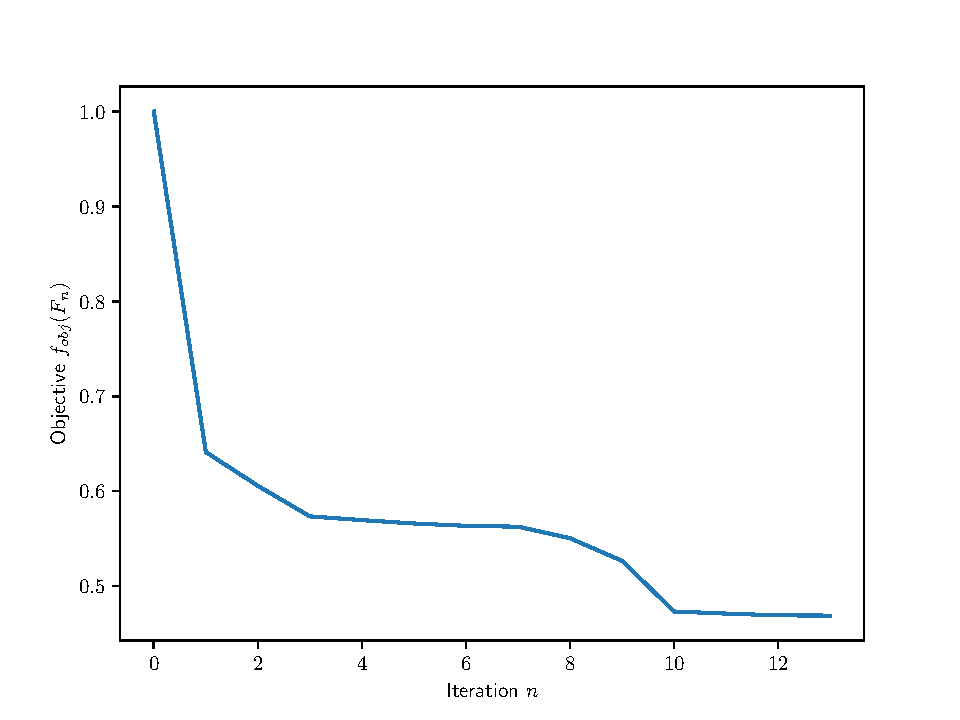
\includegraphics[width=0.8\textwidth]{figure/convergence.pdf}
    \caption{Value of \(f_{obj}\) at each iteration of the Algorithm \ref{alg:spanning-tree-greedy}.}
    \label{fig:convergence}
\end{figure}

\subsubsection{Data}

\subsubsection*{Census Blocks}

First, it is necessary to obtain \textit{shapefiles} within the area of interest, Alameda County. The most resolved unit for which we have found are \textit{Census Blocks} within \href{https://www2.census.gov/geo/tiger/TIGER2018/TABBLOCK/tl_2018_06_tabblock10.zip}{California}.

With this, we create an undirected graph \(G\) where each node represents a block within Alameda County. Values such as the \texttt{geoid} and approximate centroid (for plotting purposes) are stored at the nodes.

In addition, we use methods available from the \texttt{shapely} library to construct edges in graph \(G\) where block geometries are adjacent. Districts are considered adjacent when the intersection of their polygons contain at least \(2\) points.

\subsubsection*{Census Data}

Next, we collect other Census data of interest, in particular, \href{https://data.census.gov/table?q=P12&t=Age%20and%20Sex&g=050XX00US06001$1000000&y=2020&d=DEC%20Demographic%20and%20Housing%20Characteristics}{sex by age}, which provides population by age, sex, and census block. This may be used to determine the school-age population residing in each census block, which may be then stored at the nodes of graph \(G\).

\subsubsection*{Alameda County Data}


Property value assessments of individual parcels are available through the \href{https://data.acgov.org/datasets/2b026350b5dd40b18ed7a321fdcdba81_0/explore?location=37.716012%2C-122.135377%2C19.19}{Alameda County Data Sharing Initiative}. In particular, along with parcel \textit{shapes} and \textit{centroids}, the dataset contains 
\begin{itemize}
    \item Assessed Land Value
    \item Assessed Improvements Value
    \item \textbf{Total Assessed Value}
\end{itemize}
Since centroids are provided, we may use \textit{point-in-polygon} methods to sum the above values at the nodes of each census block.% We have already done this for larger census block groups. The resulting total land value and total land value density for Alameda County are shown in Figure \ref{fig:land-value} and \ref{fig:land-value-density}.

\begin{figure}[H]
    \centering
    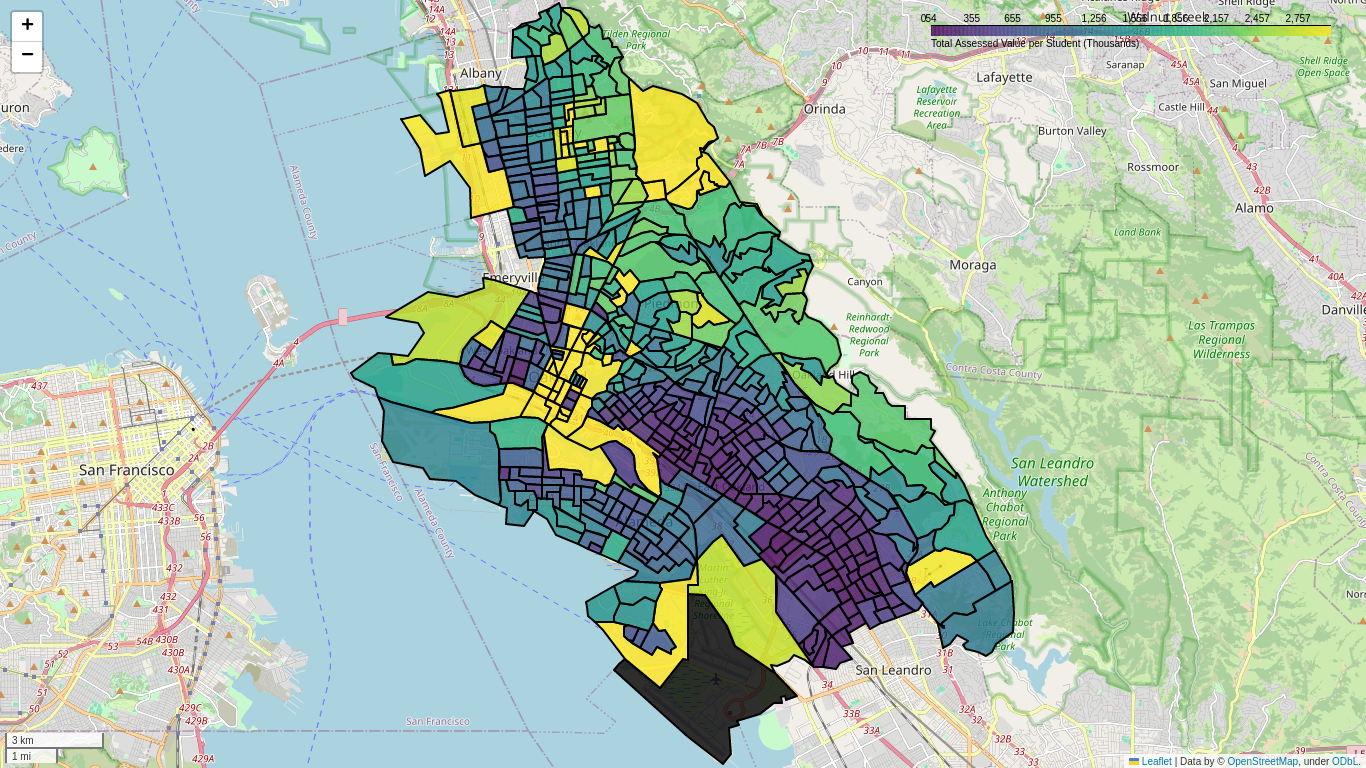
\includegraphics[width=\textwidth]{figure/districts_value.png}
    \caption{Total assessed value per student capita by census block group in our districts, measured in thousands of dollars per student.}
    \label{fig:land-value}
\end{figure}


%\begin{figure}
%    \centering
%    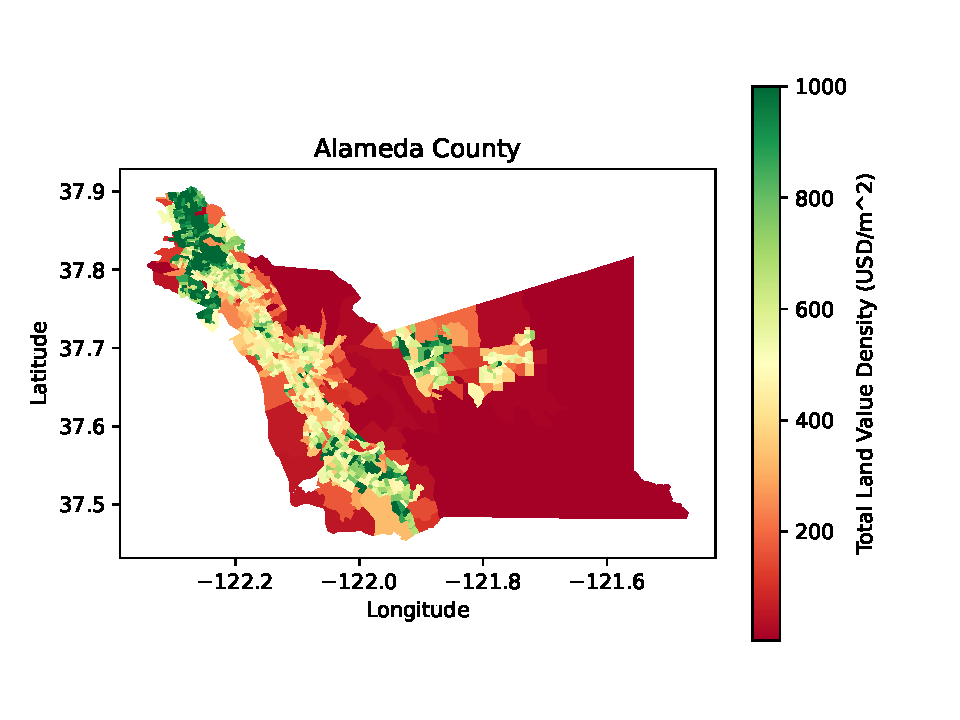
\includegraphics[scale=0.7]{figure/land_value_density.pdf}
%    \caption{Land value density by census block group in Alameda County.}
%    \label{fig:land-value-density}
%\end{figure}

\subsubsection*{Existing School District Boundaries and Creating the Initial Spanning Forest}
Existing school district boundaries are available through the \href{https://www2.census.gov/geo/tiger/TGRGDB20/tlgdb_2020_a_us_school.gdb.zip}{Census}. We may construct one of  several possible methods to create the initial spanning forest \(F\) which reflects existing school district boundaries. One simple method we employ is
\begin{enumerate}[label=(\alph*)]
    \item Compute the centroids of each Census Block
    \item Label each census block node in a copy of the graph \(G\) with the current school district that contains it using the centroid and a \textit{point-in-polygon} method
    \item Create \(n\) copies of the graph \(G_i\) for \(n\) number of districts
    \item Delete nodes in graph \(G_i\) not labeled as belonging to district \(n\)
    \item Compute the spanning tree \(T_i\) for each graph \(G_i\)
    \item Union all spanning trees \(T_i\) to get the initial spanning forest \(F_0\)
\end{enumerate}
which gives an initial spanning forest \(F_0\) on which the optimizer may minimize \(f_{\text{obj}}\). The result of steps (a)-(b) are shown in Figure \ref{fig:districts-census-blocks}. The result of step (e) is shown in Figure \ref{fig:forest-data}.

\begin{figure}[H]
    \centering
    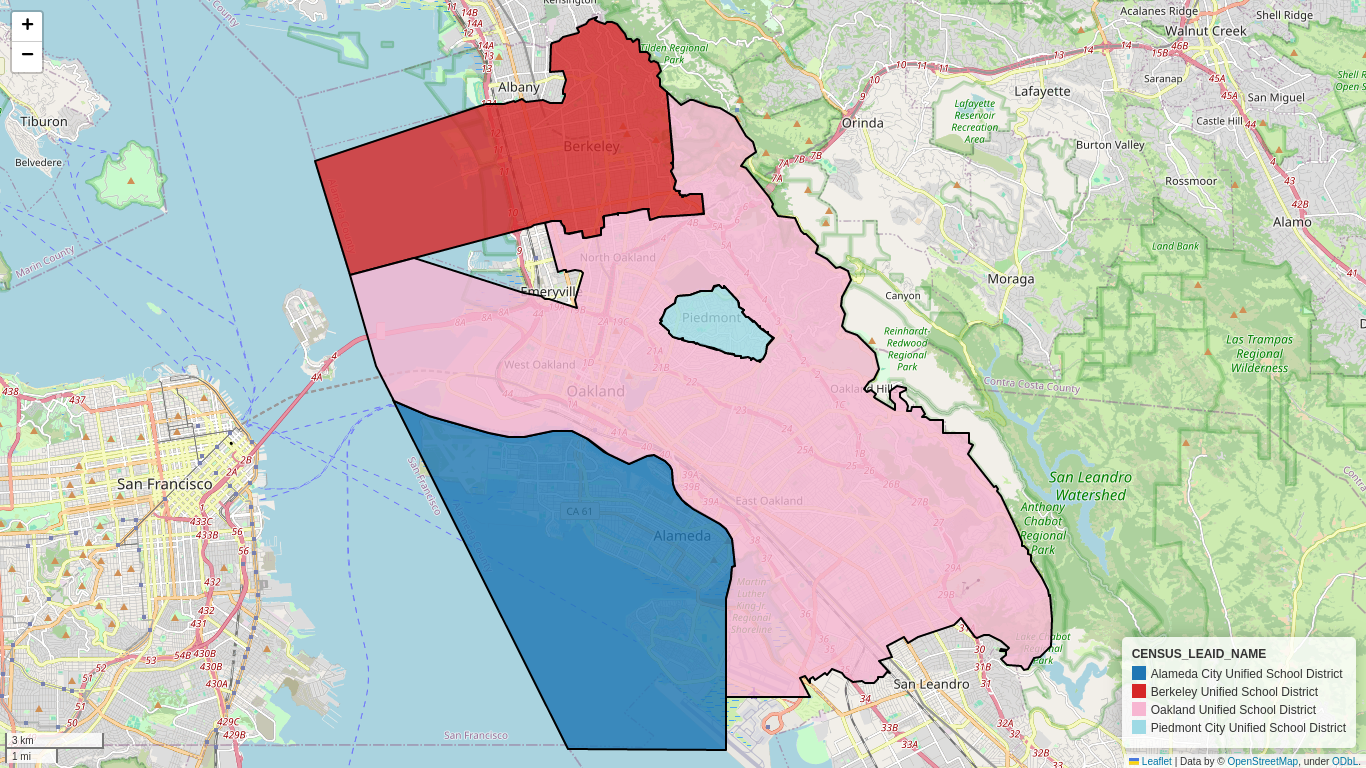
\includegraphics[width=\textwidth]{figure/districts.png}
    \caption{The map of 2020 boundaries of districts listed in Table \ref{tab:school-districts}.}
    \label{fig:districts}
\end{figure}

\begin{figure}[H]
    \centering
    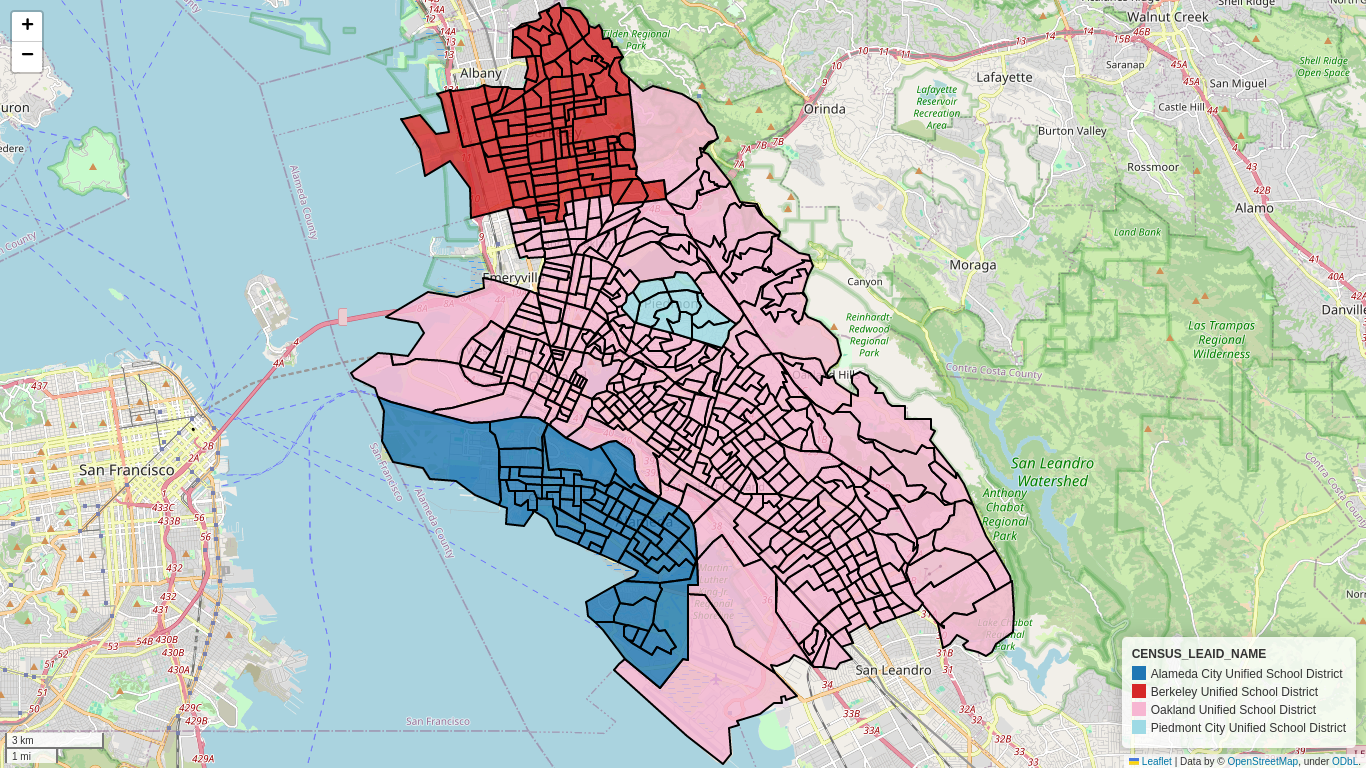
\includegraphics[width=\textwidth]{figure/districts_cb.png}
    \caption{The constituent Census blocks of districts in Table \ref{tab:school-districts} and Figure \ref{fig:districts}.}
    \label{fig:districts-census-blocks}
\end{figure}

\begin{figure}[H]
    \centering
    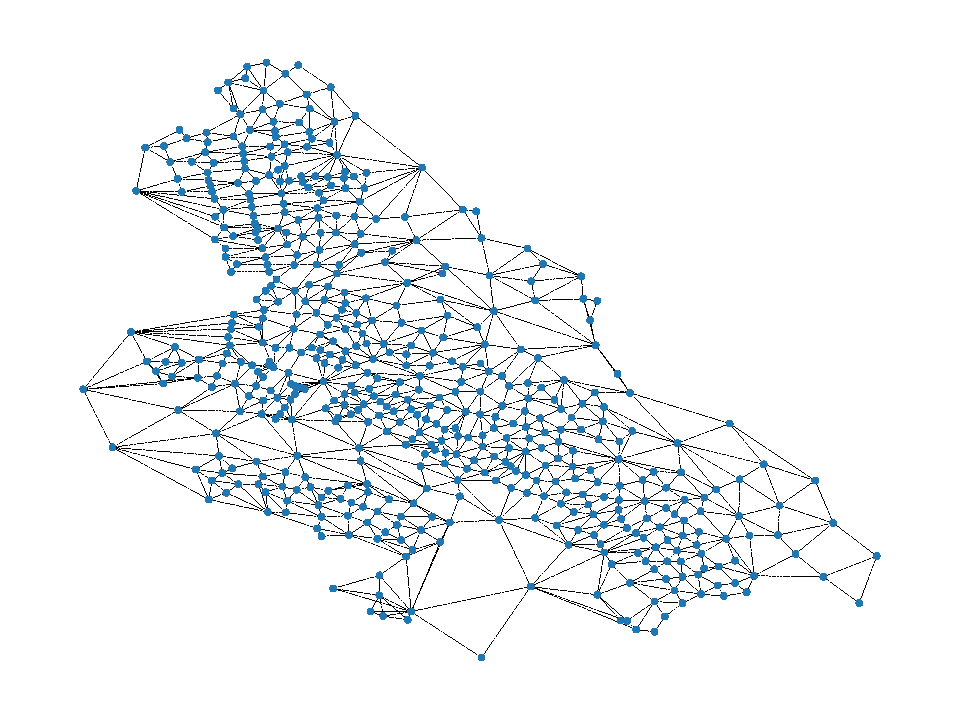
\includegraphics[width=0.8\linewidth]{figure/graph-data.pdf}
    \caption{Graph \(G\) where the centroids of census blocks are stored at nodes and edges represent adjacency.}
    \label{fig:graph-data}
\end{figure}

\begin{figure}[H]
    \centering
    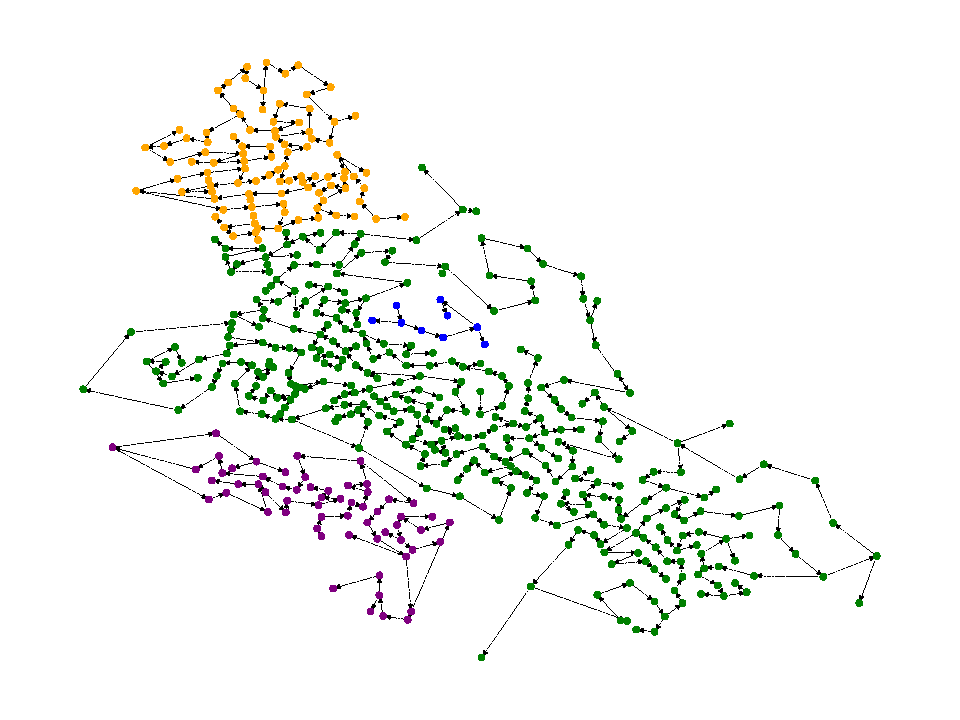
\includegraphics[width=0.8\textwidth]{figure/forest-data.pdf}
    \caption{Initial spanning forest \(F_0\) created from existing school district boundaries, where color indicates different spanning trees.}
    \label{fig:forest-data}
\end{figure}

\subsubsection{Objective Function}

The objective function we designed seeks to quantify three things, namely: Land value per student capita, district compactness, and student population. Each objective function is scaled by the initial value of the objective function on the initial spanning forest \(F_0\). These objective functions are summed into a single objective function \(f_{\text{obj}}\):

\begin{equation}
    f_{\text{obj}}(F) = f_{\text{land}}(F) + f_{\text{compact}}(F) + f_{\text{student}}(F).
\end{equation}

\subsubsection*{Land Value}
This objective function measures the mean square deviation of land value per student-age capita. Specifically,
\begin{equation}
    f_{\text{land}}(F) = \frac{1}{n \cdot f_\text{land}(F_0)} \sum^{n}_{i=1} \left(\frac{L_i}{P_i} - \frac{\hat{L_i}}{\hat{P_i}}\right)^2.
\end{equation}

\subsubsection*{Compactness}
This objective function provides a metric of ``compactness'' of each district or spanning tree \(T_i\) in the spanning forest \(F\), by dividing the length of the boundary by the area. 

Rather than compute exactly, since the centroid of each block is stored at the node, we compute a concave hull \(C_i\) around each spanning tree \(T_i\) and divide the length by the area of the resulting concave hull.
\begin{equation}\label{eq:obj-compactness}
    f_{\text{compact}}(F) = \frac{1}{n \cdot f_\text{compact}(F_0)} \sum^{n}_{i=1} \frac{\text{length}(C_i)}{\text{area}(C_i)}.
\end{equation}

\subsubsection*{Student Population Size}
This objective function measures the mean square deviation of student population size. Specifically,
\begin{equation}
    f_{\text{student}}(F) = \frac{1}{n \cdot f_\text{student}(F_0)} \sum^{n}_{i=1} \left(P_i - \hat{P}_i\right)^2.
\end{equation}
This aims to promote districts of equal size.

\section{Results and Analysis}
\subsection{Predictors of Educational Outcomes}
\subsubsection{Results}\label{sec:model-results}
First attempts to fit a linear model give the coefficients shown below in Table \ref{tab:model}.
    
\begin{table}[H]
\centering
\begin{tabular}{r|l} \hline
& \rot{\texttt{rev\_local\_total\_per\_student}} \\ \hline
\texttt{grad\_rate\_midpt}            & 0.000127 \\
\texttt{read\_test\_pct\_prof\_midpt} & 0.000312 \\
\texttt{math\_test\_pct\_prof\_midpt} & 0.000310 \\ \hline
& \rot{\texttt{rev\_state\_total\_per\_student}} \\ \hline
\texttt{grad\_rate\_midpt}            & -0.000482 \\
\texttt{read\_test\_pct\_prof\_midpt} & -0.000509 \\
\texttt{math\_test\_pct\_prof\_midpt} & -0.000703 \\ \hline
& \rot{\texttt{rev\_fed\_total\_per\_student}} \\ \hline
\texttt{grad\_rate\_midpt}            &	-0.001188 \\
\texttt{read\_test\_pct\_prof\_midpt} &	-0.003280 \\
\texttt{math\_test\_pct\_prof\_midpt} &	-0.002902\\ \hline
& \rot{\texttt{exp\_current\_instruction\_total\_per\_student}} \\ \hline
\texttt{grad\_rate\_midpt}            &	0.000767 \\
\texttt{read\_test\_pct\_prof\_midpt} &	0.002006 \\
\texttt{math\_test\_pct\_prof\_midpt} &	0.002120 \\ \hline
& \rot{\texttt{exp\_current\_supp\_serve\_total\_per\_student}} \\ \hline
\texttt{grad\_rate\_midpt}            &	-0.001370 \\
\texttt{read\_test\_pct\_prof\_midpt} &	-0.001066 \\
\texttt{math\_test\_pct\_prof\_midpt} &	-0.001706 \\ \hline
& \rot{\texttt{teachers\_total\_fte\_per\_student}} \\ \hline
\texttt{grad\_rate\_midpt}            &	-181.403511 \\
\texttt{read\_test\_pct\_prof\_midpt} &	-133.149830 \\
\texttt{math\_test\_pct\_prof\_midpt} &	-79.038562  \\ \hline
& \rot{\texttt{instructional\_aides\_fte\_per\_student}} \\ \hline
\texttt{grad\_rate\_midpt}            &  6.635612  \\
\texttt{read\_test\_pct\_prof\_midpt} &	-41.279219  \\
\texttt{math\_test\_pct\_prof\_midpt} &	-35.715050  \\ \hline
& \rot{Intercepts} \\ \hline
\texttt{grad\_rate\_midpt}            &  105.28320662  \\
\texttt{read\_test\_pct\_prof\_midpt} &	 55.52300421   \\
\texttt{math\_test\_pct\_prof\_midpt} &	 50.00160859   \\ 
\end{tabular}
\caption{Coefficients of \(\hat{\beta}\) resulting from ordinary least squares.}
\label{tab:model}
\end{table}

Evaluation on the test set of \(\mathbf{X}\) and \(\textbf{y}\) gave a mean square error of 13.72, where the mean square error is calculated as
\begin{equation*}
    \text{MSE} = \frac{1}{n} \sum_{i=1}^{n} \left(\mathbf{y}_i - \mathbf{\hat{y}}_i\right)^2.
\end{equation*}
Analysis of this model is provided in \ref{sec:model-analysis}.

\subsubsection{Analysis}\label{sec:model-analysis}
Based on the preliminary results in \ref{sec:model-results}, specifically the coefficients of Table \ref{tab:model}, we attempt here an interpretation. 

First, without proper scaling or normalization, which is planned for future work, we cannot properly interpret the relative effects of each factor in the columns of \(\mathbf{X}\). However, we may for now, pay attention to the sign of each coefficient of \(\hat{\beta}\) and reason that
\begin{itemize}
    \item Higher local funding predicts increased outcomes
    \item Higher state and federal funding predicts decreased outcomes
    \item Higher expense on instruction predicts increased outcomes
    \item Larger class sizes predict decreased outcomes
    \item Higher expense on support services predicts decreased outcomes 
    \item More instructional aides predict increased graduation rates but predicts decreased assessment scores
\end{itemize}
We stress that while the linear model may provide useful prediction, it is not sufficient to show cause--and--effect. Further discussion of this is presented in \ref{sec:model-discussion}.

%The next iteration of the model, where values are properly normalized, should also include Small Area Income Poverty Estimates, which may have stronger predictive power than already included columns in \(\mathbf{X}\).

\subsection{Optimal District Design}
\subsubsection{Results}
Applying the method described successfully minimized the objective function. A summary of changes to the districts both before and after running the optimizer may be found in Table \ref{tab:optimization-result}. Further, the resulting geographic boundaries of the new districts are shown in Figure \ref{fig:optimization-result}. Where the primary objective was to decrease the variance in tax--assessed property value per student capita, the optimizer largely succeeded, while still creating school districts that are reasonably compact.

\begin{table}[H]
    \centering
    \begin{tabular}{l|ll|ll}
         \textbf{Name}      & \multicolumn{2}{l|}{\textbf{Total Value Per Student}}    & \multicolumn{2}{l}{\textbf{Students}}\\
                            & Before                                      & After      & Before & After \\ \hline
         Berkeley Unified   & \$ 1,692,140                                & \$ 1,391,486 & 15394  & 10112 \\
         Piedmont Unified   & \$ 1,958,834                                & \$ 1,062,305 & 2987   & 1656 \\ 
         Alameda Unified    & \$ 1,158,763                                & \$ 1,085,400 & 15609  & 10034  \\ 
         Oakland Unified    & \$   931,266                                & \$ 1,054,825 & 84251  & 96439 \\ 
    \end{tabular}
    \caption{Change to district values from \(F_0\) to \(F_\text{final}\) when running Algorithm \ref{alg:spanning-tree-greedy}.}
    \label{tab:optimization-result}
\end{table}

\begin{figure}[H]
    \begin{subfigure}{\textwidth}
        \centering
        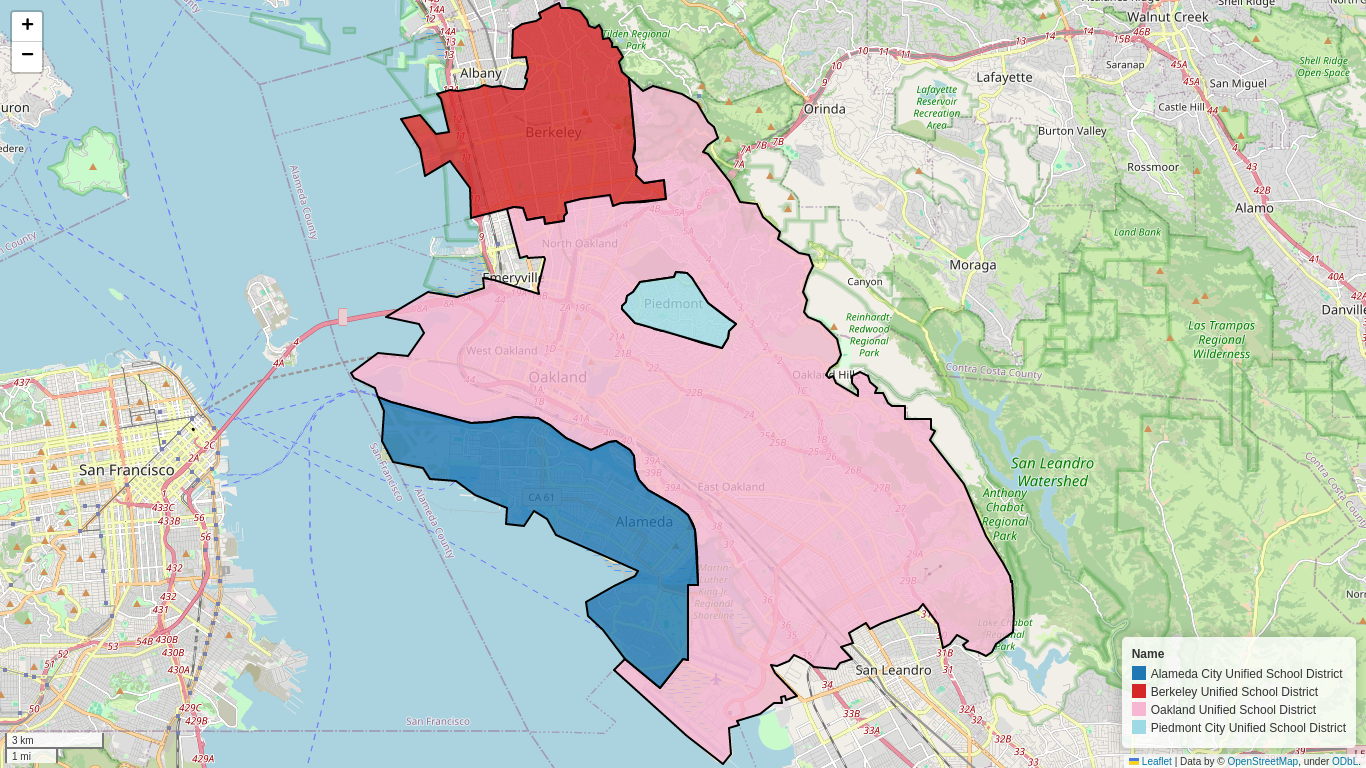
\includegraphics[width=\textwidth]{figure/result_before.png}
        \caption{District boundaries in initial spanning forest \(F_0\).}        
    \end{subfigure}
    \begin{subfigure}{\textwidth}
        \centering
        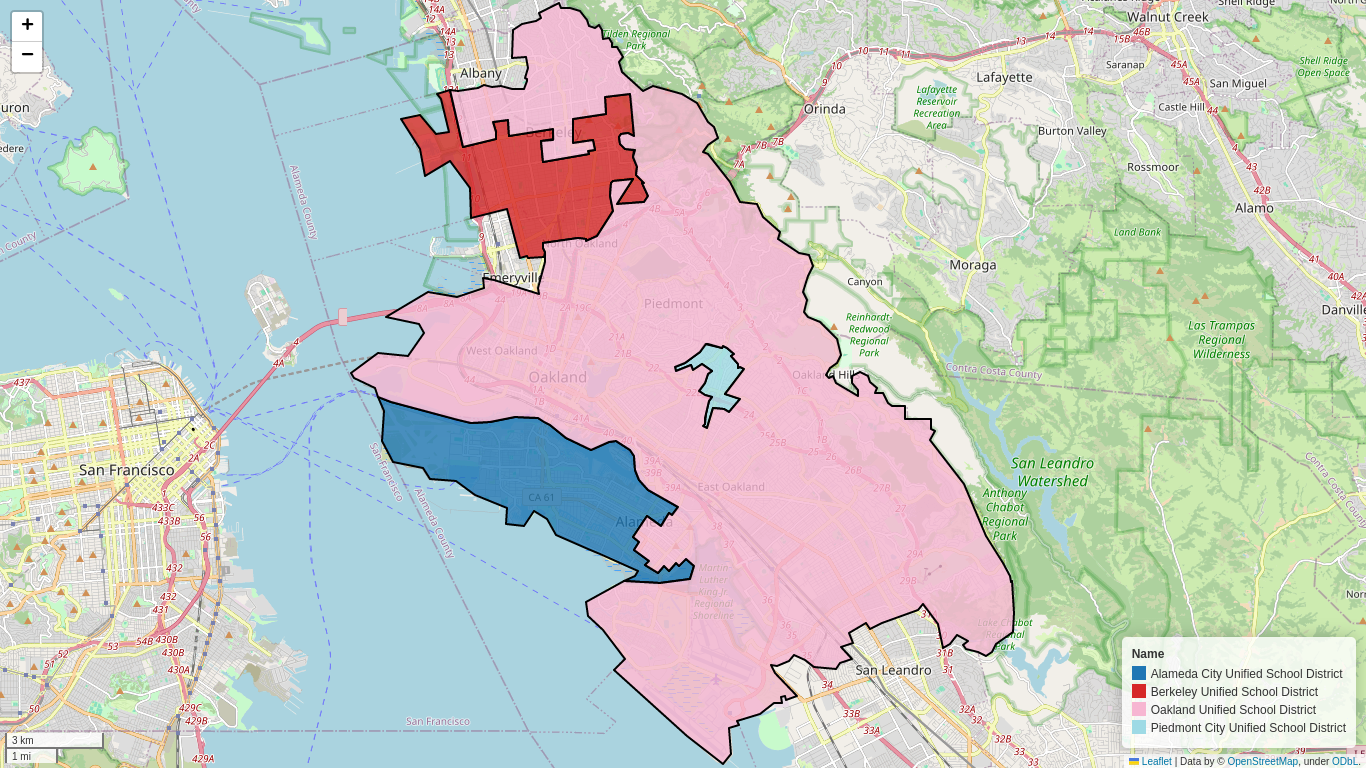
\includegraphics[width=\textwidth]{figure/result.png}
        \caption{District boundaries in final spanning forest \(F_{\text{res}}\).}        
    \end{subfigure}
    \caption{Districts boundaries of the spanning forests before and after execution of Algorithm \ref{alg:spanning-tree-greedy}.} 
    \label{fig:optimization-result}
\end{figure}

This particular result in Table \ref{tab:optimization-result} and Figure \ref{fig:optimization-result} was obtained with
\begin{equation}
    f_{\text{obj}} = f_{\text{land}} + 0.3f_{\text{compact}} + 0.2f_{\text{student}}.
\end{equation}
In experimentation, different weights on component objective functions yield different results. Planners using such a model would benefit from adjusting these weights experimentally until some acceptable result is found.

\subsubsection{Analysis}
We believe that the result provided achieves the aims set out at the beginning. However, for the particular set of districts in Table \ref{tab:school-districts}, some solutions, for various weights on the component objective functions showed consistent patterns which are discussed further in Section \ref{sec:optimizer-discussion}. We compare the result in Table \ref{tab:optimization-result} from our optimization to the most global minimum possible, in particular, if we combine all census blocks considered into a single district. This is shown in Table \ref{tab:optimization-comparision}.

\begin{table}[H]
    \centering
    \begin{tabular}{l|ll|ll} \hline
         \textbf{Name}      & \multicolumn{2}{l|}{\textbf{Total Value Per Student}}         & \multicolumn{2}{l}{\textbf{Students}}\\
                            & Value                                       & Mean Deviation  & Value  & Mean Deviation \\ \hline
         \multicolumn{5}{c}{} \\
         \multicolumn{5}{c}{\textbf{Before Optimization}} \\ \hline
         Berkeley Unified   & \$ 1,692,140                                & \$ 605,824      & 15394  & -14166 \\
         Piedmont Unified   & \$ 1,958,834                                & \$ 872,518      & 2987   & -26573 \\ 
         Alameda Unified    & \$ 1,158,763                                & \$ 72,446       & 15609  & -13951  \\ 
         Oakland Unified    & \$ 931,266                                  & \$ -155,049     & 84251  &  54690 \\ 
         \multicolumn{5}{c}{} \\
         \multicolumn{5}{c}{\textbf{After Optimization}} \\ \hline
         %\textbf{Name}      & \multicolumn{2}{l||}{\textbf{Total Value Per Student}}         & \multicolumn{2}{l}{\textbf{Students}}\\
         %                   & Value                                       & Mean Deviation  & Value  & Mean Deviation \\ \hline
         Berkeley Unified   & \$ 1,391,486                                & \$ 305,170      & 10112  & -19448 \\
         Piedmont Unified   & \$ 1,062,305                                & \$ -24,011      & 1656   & -27904 \\ 
         Alameda Unified    & \$ 1,085,400                                & \$ -916         & 10034  & -19526  \\ 
         Oakland Unified    & \$ 1,054,825                                & \$ -31,490      & 96439  &  66878 \\
         \multicolumn{5}{c}{} \\
         \multicolumn{5}{c}{\textbf{Mean Values}} \\ \hline
                            & \$ 1,086,316                                & \$ 0            & 29560  &  0 \\
    \end{tabular}
    \caption{Comparison of mean deviation of total land value per student capita before and after optimization, where the mean is the result of adding all districts into one large district and dividing by four.}
    \label{tab:optimization-comparision}
\end{table}

%Full, or even prelimary results of the optimizer in Alameda County are pending fuller analysis of the model problem in \ref{sec:model}. 

%Extremely preliminary testing of the optimizer has been carried out attempting to partition the lower 48 U.S. states into \(n\) partitions with minimum deviation in population between the \(n\) partitions. The actual implementation of the optimizer is designed such that it may be provided with a non-spanning forest \(F\), and greedily construct an initial spanning forest to then run the algorithm described in Algorithm \ref{alg:spanning-tree-greedy}. 

%Initial testing with \(n=2\) and a non--spanning forest \(F\) containing \(n=2\) nodes shows that the ability to approximate the global optimum is highly dependent on the initial spanning forest \(F\). In particular, we greedily constructed the initial spanning forest \(F\) from the exhaustive 2-pair combinations of each of the lower 48 states. One initial non--spanning forest (see Figure \ref{fig:mn-nm}), containing only the pair (Minnesota, New Mexico), resulted in a far lower objective function value than the rest. 

%Use of an early implementation of simulated annealing so far has been not promising. More often than not, the optimizer converges to a local minimum worse than, or no better than the greedy local optimum. Further testing and experimentation, both with how simulated annealing is adapted to the optimizer in Algorithm \ref{alg:spanning-tree-greedy}, as well as initial heat and cooling functions, is needed to improve the global optimum approximation. 

%\begin{figure}[H]
%    \centering
%    \includegraphics[scale=0.7]{figure/map_MN_NM.pdf}
%    \caption{Final spanning forest \(F\) when initial non-spanning forest contains only New Mexico and Minnesota, where color represents percent deviation from mean population.}
%    \label{fig:mn-nm}
%\end{figure}

%However, it may be politically desirable anyway to only converge to a local minimum. In particular, the global optimum for this given problem may likely be drastically different from the state of school districts in Alameda County today, in such a way that, if enacted, would face severe political opposition. For this reason, we hypothesize that the locally optimal solution may be sufficient, or even preferable, to the global optimum.

\section{Discussion}
\subsection{Predictors of Educational Outcomes}\label{sec:model-discussion}
\subsubsection{Limitations of Public Data}
As mentioned previously, our model is not sufficient for establishing cause--and--effect. This is because the data we have is not longitudinal, i.e. we cannot see the effect of moving between schools on individual students over time. In addition, even with longitudinal data, the effects of student self--selection into certain schools may account for the largest variance between schools. In essence, students and parents of students who are academically gifted and likely to perform well on standardized testing are more likely to self--select into schools designed for gifted children. Conversely, needy students who struggle academically are more likely to self--select (or in many cases, may be forced) into schools designed to address needy children.

With availability of longitudinal data on students, one popular approach to assess the effect of the schools themselves, rather than their ability to attract academically gifted or motivated students, is to use \textit{value--added models}. This type of model, when applied to schools, might look at the change of individual student test scores before and after changing schools, and quantify this change in aggregate for each school. However, this still does not control for student self--selection. One approach to control for this factor was explored in \parencite{angrist}, which provides useful insight into how to measure the effect the school itself has on student outcomes.

\subsection{Optimal District Design}\label{sec:optimizer-discussion}
\subsubsection{Limitations of the Optimizer}
As shown in \ref{fig:convergence}, our greedy algorithm is successful at converging to a local minimum for a given objective function. However, due to the greedy nature of the algorithm, it cannot be guaranteed that the minimum is a global minimum, or even a good approximation. Simulated annealing may help alleviate this, but it is not immediately obvious how this technique can be applied when to optimizers such as Algorithm \ref{alg:spanning-tree-greedy} that operate on graphs as a search space. Further, it is not always obvious how to create objective functions that accurately quantify desired qualities, nor how to weight them appropriately when multiple objectives are desired. This is especially true for vague concepts such as ``preserving communities'' which is often of significant consideration to district planners.

To the previous point, nearly all combinations of weights on components of \(f_{\text{obj}}\) resulted in significant changes to Piedmont Unified School District. This community is sharply distinct from the surrounding communities, having a strong history of racial exclusion\autocite{jphillips}, and having nearly twice the property value per student when compared with the surrounding Oakland district. As a result of this sharp gradient in property value, the optimizer nearly always chooses to either incorporate the entirety of Piedmont into Oakland, or, when weights on \(f_{\text{student}}\) are sufficiently high, incorporate much of Oakland into Piedmont. If such a proposal were enacted, it would almost certainly be met with strong resistance by Piedmont residents.

This hints somewhat at the fact that the most globally optimal solution in this problem is to create one large school district, as exists currently in San Francisco county. Though this is always the most optimal choice for any set of districts in reducing inequality, and where the most legal protection exists against segregation (compared with segregation via separate school districts), whether or not political will exists (or how to foster it) to attempt enacting such optimal solutions (or even the approximately optimal results presented here) is a separate question which our models cannot hope to address.

\subsubsection{Limitations of our Data}
Some consideration should also be given to the quality of our data. We believe the general approach of using Census Blocks with Algorithm \ref{alg:spanning-tree-greedy} is overall sound. However, in particular for our tax--assessment data, we feel that we ought to note that directly comparing land--value between districts is not exactly the same as the actual local revenue that is generated within districts. In particular, many of the actual funding amounts following the enactment of Proposition 13 greatly complicate things.

Following the enactment of Proposition 13, actual funding from local sources is now fixed through the \href{https://www.cde.ca.gov/fg/aa/lc/lcffoverview.asp}{Local Control Funding Formula} (LCCF), where previously school districts were unrestricted in setting property tax rates. This means, in practice, that local school districts cannot fully set their own property tax rates. To circumvent this, many communities who wish to better fund their school district, including Piedmont, implement a \textit{parcel tax}, which are fixed taxes on land parcels not in proportion to actual fixed values, effectively circumventing Proposition 13.

Thus, an improved version of the model might implement these formulas and considerations (including parcel taxes). However, outside of California, the approach to control for this is much simpler, where districts continue to set their own property tax rates. 

\newpage
\section{Appendix}
\subsection{Algorithms}
\begin{algorithm}[H]
\caption{Perform local search on the spanning forest using steepest descent}\label{alg:spanning-tree-greedy}
\begin{algorithmic}
\Input
\Desc{\(f_{obj}\)}{Objective function}
\Desc{\(G\)}{Undirected graph with nodes containing geographic regions and edges representing shared borders}
\Desc{\(F\)}{Directed graph which is a spanning forest of graph \(G\)}
\Desc{\(k_{\text{max}}\)}{Maximum iterations}
\EndInput
\Output
\Desc{\(F\)}{Locally optimized spanning forest}
\EndOutput
\State \(k \gets 0\)
\While{\(k < k_{\text{max}}\)}
\State \(k \gets k+1\)
\State \(val \gets f_{obj}(F)\)
\State \(weight \gets \infty\)
\State \(E \gets \emptyset\)
\ForAll{trees \(T \in F\)}
\ForAll{nodes \(N \in T_i\)}
\ForAll{adjacent nodes \(N^{adj} \in (\Call{adjacent}{G, N_i} \cap N)\)}
\State \(F_{c} \gets \Call{Copy}{F_i}\)
\State \(\Call{DeleteEdgesTo}{F_{c}, N^{adj}_i}\)
\Comment{Test the result of adding \(N^{adj}_i\) to the tree \(T_i\)}
\State \(\Call{AddEdge}{F_{c}, N_i, N^{adj}_i}\)
\State \(f_{eval} \gets f_{obj}(F_{c})\)
\If{\(f_{eval} < val\)}
\State \(weight \gets f_{eval}\)
\State \(E \gets \{N_i, N^{adj}_i\}\)
\EndIf
\EndFor
\EndFor
\EndFor
\If{\(weight > 0\)}
\Comment{There are no optimal choices in this neighborhood.}
\State \Return \(F\)
\EndIf
\State \(val \gets weight\)
\State \(\Call{DelteEdgesTo}{F, E_1}\)
\State \(\Call{AddEdge}{F, E_1, E_2}\)
\EndWhile
\State \Return \(F\)
\end{algorithmic}
\end{algorithm}

\newpage
\section{References}
\printbibliography[heading=none]

\end{document}
